\documentclass[11pt]{article}

\usepackage[utf8]{inputenc}
\usepackage[T1]{fontenc}
\usepackage[margin=1in]{geometry}
\usepackage{amsmath,amssymb}
\usepackage{booktabs}
\usepackage{longtable}
\usepackage{graphicx}
\usepackage{xcolor}
\usepackage{siunitx}
\usepackage[hidelinks]{hyperref}
\usepackage[numbers,sort&compress]{natbib}
\usepackage{caption}
\usepackage{array}
\usepackage{makecell}
\usepackage{multirow}
\captionsetup{font=small,labelfont=bf}

\newcommand{\minus}{\ensuremath{-}}
\newcommand{\superior}{\textsc{superior}}
\newcommand{\inconclusive}{\textsc{inconclusive}}
\newcommand{\equivalent}{\textsc{equivalent}}
\newcommand{\inferior}{\textsc{inferior}}

\title{\bfseries How much viral capability do genomic language models add over conventional predictors?
}

\author{%
Aris Karatzikos$^{1,2}$ \quad Xiang Han$^{3}$ \quad Ilias Georgakopoulos-Soares$^{1,*}$\\[6pt]
\begin{minipage}{0.92\textwidth}
\centering\small
$^{1}$Division of Pharmacology and Toxicology, College of Pharmacy, The University of Texas at Austin, Dell Pediatric Research Institute, Austin, TX, USA\\[2pt]
$^{2}$Department of Computer Science, College of Natural Sciences, The University of Texas at Austin, Austin, TX, USA\\[2pt]
$^{3}$External Collaborator\\[2pt]
$^{*}$Correspondence: \href{mailto:ilias@austin.utexas.edu}{ilias@austin.utexas.edu}
\end{minipage}}
\date{}

\begin{document}
\maketitle

\begin{abstract}
\noindent
We evaluate the viral capabilities attributed to genomic language models by measuring them against conventional sequence predictors on the same data. On nine published viral classification benchmarks we fit seven conventional methods, from $k$-mer models and supervised convolutional networks to transfer of the label of the closest training sequence, and compare the best of them against a foundation model selected on the development split. We then ask whether these benchmarks are fair tests of generalization, by searching each test set against its own training data for homology the benchmark's construction left behind. Applying a second round of DNA homology filtering removes a large part of the measured performance, for the conventional methods and for the foundation models alike, which locates most of a published score in sequences that have a close training relative. On what survives, the models retain more of their score than the conventional methods do, a gap the composition of the comparator partly explains and which a direct test does not resolve. Filtering at the DNA level still leaves homology in place, since a translated search finds a relative for most of the sequences a DNA search calls distant. As these models improve and their potential for misuse is assessed, what matters is the capability they add beyond methods that are already cheap and available, measured on benchmarks whose difficulty is known. We give that measurement for nine benchmarks and a protocol for obtaining it on new ones.
\end{abstract}

\section{Introduction}

Genomic language models trained by self supervision on large DNA corpora \citep{nguyen2024evo,brixi2025evo2,dallatorre2024nt,zhou2024dnabert2,nguyen2023hyenadna} are applied to viral classification tasks with direct relevance to annotation, surveillance and capability assessment. Virus specialized derivatives report strong performance on human virus properties such as host range, pathogenicity and transmissibility \citep{dutta2026hvilm,dip2024patholm}, and those numbers now inform assessments of the misuse potential of open weight biological models and proposals to remove hazardous capabilities from released weights \citep{black2026safeguards}.

Reading a benchmark score as a capability estimate requires two things of the benchmark. The first is a comparator, because a score is only informative relative to what is already available. Work across genomics has found that tuned supervised baselines are competitive with genomic foundation models on many tasks \citep{xu2025specialized,patel2024dart,ledneva2026geneb}, and in protein function prediction, viral classification and enzyme annotation the label of the closest training sequence is a standard and strong comparator \citep{kulmanov2020deepgoplus,sanderson2023proteinfer,cafahomology,borozan2015viral,fahmy2026retrieval,sathyamoorthy2026ec}. The second is a test set whose difficulty is understood. \citet{petti2023graphpart} show that homology partitioning frequently leaves more similarity between splits than intended, \citet{spectra2024} argue that generalization is better characterized across a spectrum of train to test overlap than at a single cutoff, and \citet{rafi2026hashfrag} demonstrate that residual relatedness inflates apparent performance in genome trained models. Translated search is established in viral machine learning as a way of detecting relationships that nucleotide search misses \citep{perelygin2025host,virhunter2022}.

This paper has two parts. The first audits the nine benchmarks as published, asking what a foundation model adds over the best of seven conventional predictors. The second asks what survives when we search each test set against its own training split and withhold the sequences that still have a detectable relative, which changes both what the benchmarks measure and which side is ahead. We apply that search at two sensitivities, first at the DNA level and then in six frame translation, since nucleotide similarity decays through synonymous substitution while protein similarity persists.

Relatedness is frequently the reason viral prediction works, and we treat it as signal rather than as a defect. Viruses in one taxonomic group often share hosts, and among Viral RefSeq genera carrying host annotation, 73 percent are host consistent \citep{phagehost2025}. A predictor that transfers a label from an informative relative is doing what it was built to do, which is how \citet{mollentze2021} frame the same problem for human infecting viruses. Our question is what a given benchmark can separate, so that a claim is matched to the evidence behind it.

The motivation is practical. As these models improve, decisions about release, safeguards and capability removal will rest on benchmark numbers. A number is only actionable if it reflects capability the model uniquely provides, rather than capability a $k$-mer model or a sequence lookup would supply at negligible cost, and if the test set is known to be hard in the way the claim requires. We provide both measurements for nine current benchmarks, and the protocol is cheap enough to apply to new ones before they are adopted.

\section{Methods}

\subsection{Benchmarks}

We audit nine published viral classification tasks drawn from three sources.

Six come from HVUE, the evaluation suite released with the virus specialized model HViLM \citep{dutta2026hvilm}. They cover three phenotypes, namely host tropism, which asks whether a virus infects humans, pathogenicity, and transmissibility. Each phenotype ships in a stricter and a looser split configuration and we audit both, since a user of the suite is offered both. Only host tropism names its configurations by sequence identity, \textsc{hard\_70} and \textsc{standard\_95}, where identity is the percentage of aligned positions that match between a test and a training sequence, so the stricter split is intended to place more evolutionary distance between train and test. Pathogenicity and transmissibility label theirs \textsc{hard} and \textsc{standard} without stating a threshold, and additionally ship a temporal split that we do not use. No configuration ships a description of how it was partitioned. We therefore audit the released splits as given, and we neither choose these thresholds nor re-partition, since our aim is to characterise what the splits contain rather than to restate how they were built.

One task we built ourselves from Virus-Host~DB \citep{mihara2016vhdb}, hereafter VHDB. It asks the same host tropism question but draws its negatives from within the same viral family as its positives, so a predictor cannot succeed by recognising family membership alone. It is the only benchmark in the study that ships a genome identifier and a lineage label for every sequence.

Two come from GUE \citep{zhou2024dnabert2}, a general genomic benchmark suite. One is phage fragment classification, which asks whether a sequence comes from a bacteriophage, and the other is SARS-CoV-2 variant classification, reported here on de duplicated sequences after we found that 10.66 percent of its test sequences appear verbatim in its training split.

All sequences are cut to 1{,}000\,bp windows. Sizes and class balance are in Supplementary Table~S1.

\subsection{Models}

We evaluate five genomic language models chosen to span the design space. Nucleotide Transformer v2 at 500M parameters \citep{dallatorre2024nt} and DNABERT-2 \citep{zhou2024dnabert2} are general purpose masked language models over nucleotide and byte pair tokens respectively. GENA-LM \citep{fishman2025genalm} extends that family to longer context.
 HyenaDNA \citep{nguyen2023hyenadna} replaces attention with an implicit long convolution, giving a different inductive bias at similar scale. HViLM \citep{dutta2026hvilm} is specialized to viral genomes and is the model whose reported viral capabilities motivate the audit. Evo~2 \citep{brixi2025evo2} is included by frozen probing only, because full fine tuning exceeded our compute budget.

Each model is fine tuned from its pretrained base under one uniform protocol with a learning rate grid, three seeds and a development selected epoch whose optimum we verify is interior. For every benchmark the model identity and its learning rate are both selected by mean development split MCC over three seeds, and the selected model is then held fixed across all filtering levels, so selection uses no test set quantity (Supplementary Table~S3). As a check we also report a symmetric variant in which the best model and the best conventional predictor are both re selected inside each bootstrap replicate, which applies the same selection rule to both sides and agrees with the development selected model on every benchmark.

\subsection{The baseline}

The comparator is the best of seven conventional predictors on the population being scored, each fit on the benchmark's own training split with hyperparameters chosen on its development split. Taking the best rather than the average asks whether a foundation model beats the strongest cheap method available.

\begin{enumerate}\itemsep2pt
\item \textbf{$k$-mer logistic} and \textbf{$k$-mer GBT}. Nucleotide 3 to 6-mer frequencies into $L_2$ regularized logistic regression and into gradient boosted trees. These capture base composition and short motif usage.
\item \textbf{Amino acid composition GBT}. Amino acid $k$-mer frequencies of the six frame translation into gradient boosted trees, capturing composition at the protein level.
\item \textbf{CNN ladder}. A searched supervised convolutional baseline spanning dilated, U-Net and ResNet architectures from 0.04M to 9.4M parameters, with kernel, dilation, capacity and learning rate swept and the cell chosen on development, following \citet{xu2025specialized}. This is the strongest purely supervised model we fit.
\item \textbf{Transformer ladder}. A from scratch supervised transformer, included so that a transformer trained only on the task appears alongside one that was pretrained.
\item \textbf{Nearest neighbour lookup}. The label of the top training hit under nucleotide MMseqs2 search \citep{steinegger2017mmseqs2}, which measures how far pure relatedness transfer gets on its own.
\item \textbf{Taxonomy prior}. The majority training label of the test sequence's genus, backing off to species and then family, which measures how far lineage membership alone gets. Genus labels ship with VHDB. On the two host tropism benchmarks we recover them by MMseqs2 alignment to RefSeq viral and normalize to genus rank through the NCBI taxonomy, which raises agreement with VHDB's own labels from 87.6 to 99.9 percent. Native and recovered labels are never pooled, and the remaining six benchmarks support neither.
\end{enumerate}

Each predictor's score is averaged over its training seeds before the best is taken, so the comparator gains no best of seeds advantage the model does not also receive. Nearest neighbour lookup requires a nucleotide match in training, so it applies on the published test sets and is reported as unavailable on the filtered populations defined by the absence of that match.

\subsection{Homology filtering}

For each test sequence we search the benchmark's own training split with a fixed protocol, chosen as the most permissive detection setting that still returns meaningful alignments and never relaxed to enlarge a population. It is MMseqs2 \texttt{easy-search} \citep{steinegger2017mmseqs2}, nucleotide \texttt{--search-type 3} and translated six frame \texttt{--search-type 2 -s 7.5}, with \texttt{--min-seq-id 0.30 -c 0.10 --cov-mode 2 -e 1e-3}, on both strands. Profile based search \citep{eddy2011hmmer,steinegger2019hhsuite} and dedicated protein aligners \citep{altschul1990blast,buchfink2021diamond} are more sensitive still, and would find more of the relationships we report.

This defines three nested populations. \textsc{l0} is the published test set. \textsc{l1} keeps the test sequences with no detectable nucleotide relative in training. \textsc{l2} keeps those with no detectable translated relative either.

\subsection{Intervals and verdicts}

The reported quantity is the difference in MCC between the selected model and the best conventional predictor on the population being scored. Intervals come from resampling the test sequences with replacement, 5{,}000 replicates, with the best predictor re selected inside each replicate and a training seed drawn at random for every method so that seed variance is propagated. Point estimates average three fine tuning seeds.

A difference is called \superior{} when the whole interval lies above zero, \inferior{} when it lies below, and \equivalent{} when the whole interval lies inside a pre declared margin of 0.02~MCC. It is \inconclusive{} when the interval spans zero and also runs past the margin, which is the outcome an underpowered population returns and which we treat as an absence of evidence. The equivalence rule is a 95 percent interval inside margin criterion rather than a two one sided test at $\alpha=0.05$, and we name it that way because the two do not coincide in general. Where we test a family of hypotheses we report Benjamini-Hochberg adjusted values and treat only those as evidence.

\section{Results}

\subsection{What the models add on the published benchmarks}
\label{sec:performance}

On the published test sets the foundation models add little, and what they add depends on the task. Resampling test sequences, the model is ahead with its interval clear of zero on two benchmarks, a conventional predictor is ahead on two, the two are equivalent within the margin on two, and three do not resolve (Figure~\ref{fig:performance}A, Table~\ref{tab:headtohead}). A conventional predictor therefore matches or beats the model on four of the nine. The two clearest model wins are NT-v2 on phage classification and HViLM on the stricter host tropism split. The two clearest conventional wins are on SARS-CoV-2 variant classification, where a boosted $k$-mer model comes out ahead, and on the looser host tropism split, where label lookup does.

Those verdicts resample test sequences. Resampling the parent genomes the sequences were cut from is the more conservative unit and most of the verdicts do not survive it, with six moving to inconclusive and the differences themselves unchanged (Table~\ref{tab:headtohead}). We report both and treat a difference as established only where it holds under the genome unit.

Which conventional method wins varies across the nine. Label lookup wins on three of the published test sets, a boosted $k$-mer model on three, a convolutional network on two and a taxonomy prior on one. A single cheap method would therefore understate what is available, which is why the comparator is the best of several.

% <<< GENERATED table_headtohead (do not edit by hand)
\begingroup\scriptsize\setlength{\tabcolsep}{1.9pt}
\begin{longtable}{ll l rr r ll r}
\caption{\textbf{Model and best baseline MCC, their difference, and bootstrap intervals.} \textsc{l0} is the published test set, \textsc{l1} the sequences with no detectable nucleotide relative in training. The model and its learning rate are selected on the development split and held fixed. Intervals are 95 percent bootstrap intervals. The sequence interval resamples test sequences; the genome interval resamples the parent genomes they were cut from, holding the same scores, so the difference itself is identical under both. A genome interval is not estimable for the two GUE benchmarks, which ship no provenance. Verdicts are \textsc{sup} when the interval lies above zero, \textsc{inf} when below, \textsc{eqv} when wholly inside the 0.02~MCC margin, and \textsc{inc} otherwise.}
\label{tab:headtohead}\\
\toprule
Benchmark & Reg. & Model & model & base. & excess & sequence 95\% CI & genome 95\% CI & $n$ \\
\midrule\endfirsthead
\toprule Benchmark & Reg. & Model & model & base. & excess & sequence 95\% CI & genome 95\% CI & $n$ \\ \midrule \endhead
GUE phage & \textsc{l0} & NT-v2 & 0.920 & 0.813 & +0.107 & $[+0.05, +0.12]$ \textsc{sup} & not estimable & 4,630 \\
 & \textsc{l1} & NT-v2 & 0.891 & 0.770 & +0.120 & $[+0.05, +0.14]$ \textsc{sup} & not estimable & 2,874 \\
\addlinespace
HVUE host tropism \textsc{hard\_70} & \textsc{l0} & HViLM & 0.723 & 0.623 & +0.100 & $[+0.05, +0.14]$ \textsc{sup} & $[-0.02, +0.22]$ \textsc{inc} & 51,187 \\
 & \textsc{l1} & HViLM & 0.285 & 0.092 & +0.194 & $[+0.11, +0.26]$ \textsc{sup} & $[+0.06, +0.35]$ \textsc{sup} & 11,994 \\
\addlinespace
VHDB within family & \textsc{l0} & HViLM & 0.704 & 0.681 & +0.023 & $[-0.03, +0.07]$ \textsc{inc} & $[-0.08, +0.13]$ \textsc{inc} & 3,754 \\
 & \textsc{l1} & HViLM & 0.495 & 0.175 & +0.320 & $[+0.19, +0.44]$ \textsc{sup} & $[-0.06, +0.60]$ \textsc{inc} & 1,200 \\
\addlinespace
HVUE pathogenicity \textsc{hard} & \textsc{l0} & HViLM & 0.804 & 0.799 & +0.005 & $[-0.03, +0.03]$ \textsc{inc} & $[-0.04, +0.03]$ \textsc{inc} & 1,792 \\
\addlinespace
HVUE pathogenicity \textsc{std} & \textsc{l0} & DNABERT-2 & 0.810 & 0.809 & +0.001 & $[-0.02, +0.01]$ \textsc{eqv} & $[-0.02, +0.01]$ \textsc{inc} & 6,651 \\
 & \textsc{l1} & DNABERT-2 & -0.027 & 0.153 & -0.181 & $[-0.56, +0.16]$ \textsc{inc} & $[-0.63, +0.14]$ \textsc{inc} & 41$^{*}$ \\
\addlinespace
HVUE transmissibility \textsc{std} & \textsc{l0} & HViLM & 0.693 & 0.693 & -0.001 & $[-0.02, +0.01]$ \textsc{eqv} & $[-0.02, +0.01]$ \textsc{inc} & 12,728 \\
 & \textsc{l1} & HViLM & 0.464 & 0.295 & +0.169 & $[-0.36, +0.38]$ \textsc{inc} & $[-0.33, +0.38]$ \textsc{inc} & 41$^{*}$ \\
\addlinespace
GUE \textsc{virus\_covid} & \textsc{l0} & HViLM & 0.697 & 0.719 & -0.023 & $[-0.04, -0.01]$ \textsc{inf} & not estimable & 9,168 \\
\addlinespace
HVUE transmissibility \textsc{hard} & \textsc{l0} & HViLM & 0.664 & 0.689 & -0.024 & $[-0.07, +0.01]$ \textsc{inc} & $[-0.07, +0.01]$ \textsc{inc} & 2,497 \\
 & \textsc{l1} & HViLM & 0.652 & 0.412 & +0.240 & $[-0.15, +0.47]$ \textsc{inc} & $[-0.15, +0.47]$ \textsc{inc} & 55$^{*}$ \\
\addlinespace
HVUE host tropism \textsc{std\_95} & \textsc{l0} & HViLM & 0.560 & 0.619 & -0.059 & $[-0.08, -0.04]$ \textsc{inf} & $[-0.13, +0.01]$ \textsc{inc} & 50,817 \\
 & \textsc{l1} & HViLM & 0.333 & 0.151 & +0.183 & $[+0.08, +0.27]$ \textsc{sup} & $[-0.13, +0.42]$ \textsc{inc} & 11,124 \\
\bottomrule
\end{longtable}
\vspace{-8pt}\par\noindent\footnotesize Every model and conventional predictor on every benchmark and population is in Supplementary Table~S2. An asterisk marks a population holding fewer than 100 sequences, which supports no summary claim.
\endgroup
% >>> GENERATED table_headtohead

\begin{figure}[t]
\centering
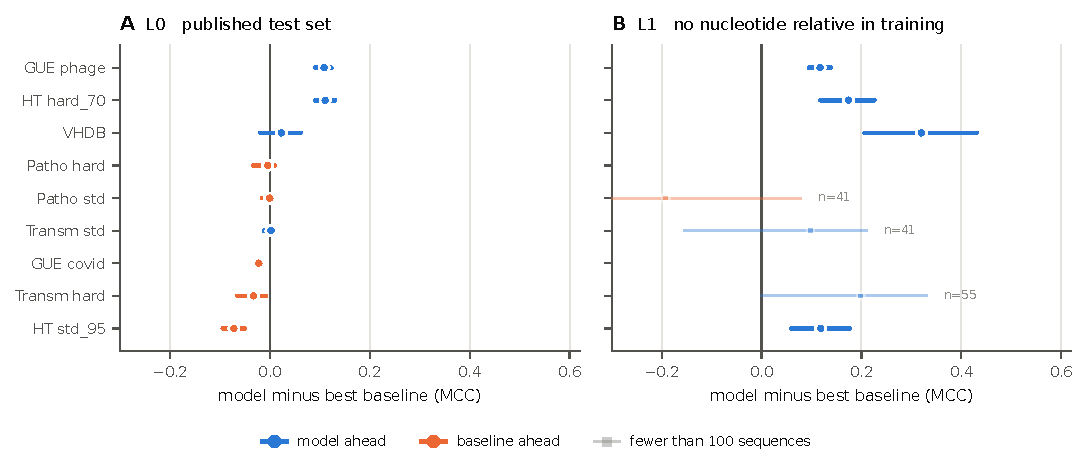
\includegraphics[width=\textwidth]{figures/fig1_performance.pdf}
\caption{\textbf{Model MCC minus best baseline MCC.} \textbf{A}, the published test set (\textsc{l0}). \textbf{B}, the test sequences with no detectable nucleotide relative in training (\textsc{l1}). One row per benchmark, ordered identically in both panels. Points are the difference in MCC, bars are 95 percent bootstrap intervals over test sequences. Populations holding fewer than 100 sequences are drawn as open squares and labelled with their size.}
\label{fig:performance}
\end{figure}

\subsection{What survives DNA homology filtering}
\label{sec:divergent}

Each of these benchmarks was built by searching candidate sequences against training sequences at the DNA level and removing what matched. We repeated that search with a permissive setting and kept only the test sequences that still had no detectable nucleotide relative in training. The amount that survives varies widely, from most of the phage benchmark to none at all for SARS-CoV-2 variants (Figure~\ref{fig:filters}).

The first result is that performance falls sharply on what remains, for both sides. On host tropism the best conventional predictor drops from 0.62 to 0.09~MCC and the model from 0.72 to 0.29. On VHDB the conventional predictor drops from 0.68 to 0.18 and the model from 0.70 to 0.50 (Figure~\ref{fig:collapse}). Most of what these benchmarks measure therefore comes from test sequences that retain a close training relative, and the benchmark's own filtering step left those sequences in place.

The second result is that the model leads on every filtered population large enough to evaluate (Figure~\ref{fig:performance}B). Three further benchmarks retain only a few dozen sequences, which we report and exclude from any summary.

The models therefore degrade more gracefully than the conventional methods on these populations. Three things separate that statement from a claim about capability, and we measured all three.

The first is the composition of the comparator. On the benchmarks with the largest shift, the winning conventional method on the published test set is label lookup or a taxonomy prior, both of which transfer a label from a related training sequence. The filtered population is defined by the absence of the match label lookup requires, so the comparator falls back to a weaker method, while lineage membership becomes less informative for the taxonomy prior. Phage classification is the control, since its comparator is a convolutional network at both levels, nothing is removed by construction, and the model's margin is close to unchanged.

The second is that the change itself does not reach significance. We tested it directly, as the difference between the two margins, resampling the published population and carrying each sequence's membership of the filtered subset. Across ten tests under two definitions of the comparator, none survives correction for multiple testing (Supplementary Table~S7).

The third is the resampling unit. Under genome resampling only host tropism \textsc{hard\_70} at \textsc{l1} keeps an interval clear of zero, and that result holds under every assumption we impose about dependence among the sequences whose source genome could not be recovered (Supplementary Tables~S4 and~S5).

\begin{figure}[t]
\centering
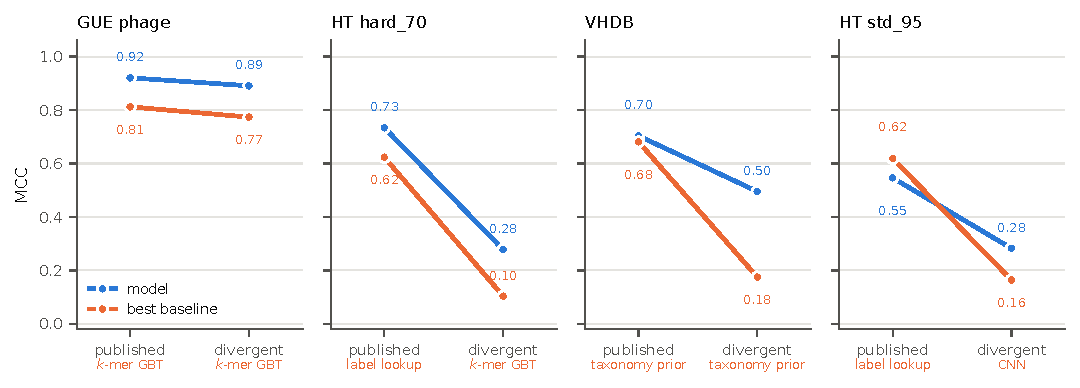
\includegraphics[width=\textwidth]{figures/fig2_baseline_collapse.pdf}
\caption{\textbf{MCC of the model and of the best baseline, before and after DNA homology filtering.} The four benchmarks retaining at least 100 filtered sequences. Lines join the published test set to the filtered population. The conventional method holding the baseline at each level is named below the axis.}
\label{fig:collapse}
\end{figure}

\subsection{DNA filtering leaves homology in place}
\label{sec:translated}

Nucleotide similarity decays through synonymous substitution while protein similarity persists, so a sequence that a DNA search calls distant can remain clearly related once translated. Searching the filtered populations again in six frame translation finds a relative for between about two thirds and almost all of them, depending on the benchmark (Figure~\ref{fig:filters}).

Whether that retained relationship is what the models are using is a separate question, and we find no consistent evidence that it is. Splitting each filtered population into the sequences that do and do not acquire a translated relative gives a pooled difference whose interval spans zero. The difference is positive in 8 of 10 model by benchmark cells, which a sign test does not separate from chance at $p=0.109$, and the clearest single positive contrast belongs to a $k$-mer logistic regression, which has no reading frames (Supplementary Table~S6).

A DNA filtered benchmark therefore measures performance on sequences that are distant at the nucleotide level, which for surveillance and annotation is frequently the operationally relevant setting. Characterising performance on sequences with no detectable evolutionary relationship needs the translated filter, and no benchmark resolves the difference it contains at that level. The two host tropism sets still hold thousands of sequences there, so sample size is not the only obstacle; on host tropism \textsc{hard\_70} the difference is $+$0.108 with a sequence interval of $[-0.03, +0.23]$ and a genome interval of $[-0.07, +0.40]$ (Supplementary Tables~S1 and~S4). The remaining benchmarks retain a few dozen sequences or fewer.

\begin{figure}[t]
\centering
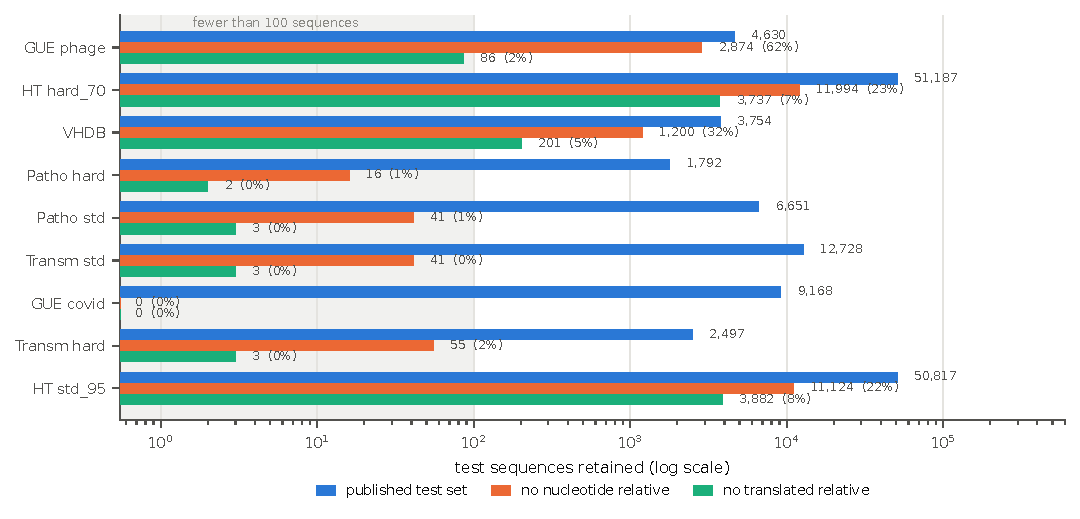
\includegraphics[width=\textwidth]{figures/fig3_what_filters_remove.pdf}
\caption{\textbf{Test sequences retained at each filtering level.} Per benchmark, the published test set, the sequences with no detectable nucleotide relative in training, and the sequences with no detectable six frame translated relative either. Percentages are of the published test set. Log axis, shading below 100 sequences.}
\label{fig:filters}
\end{figure}

\section{Discussion}

Across nine viral benchmarks, the capability a genomic language model adds over conventional predictors is task specific and frequently small. On four of the nine a tuned $k$-mer model, a small supervised convolutional network or a lookup of the closest training sequence matches or beats the foundation model. A viral benchmark score is therefore most informative when the best conventional predictor on the same data is reported beside it, since on these tasks the two are often the same number.

Most of what these benchmarks measure rests on training relatives that their construction left in place. When we apply a second round of DNA homology filtering, performance falls by a large margin for the conventional methods and for the models alike. This locates the bulk of a published score in test sequences that have a close relative in training, and it means a score quoted without a stated similarity regime describes an easier task than the phenotype name suggests.

The models lead on what survives that filtering, and the cleanest reading of this is that they degrade more gracefully than label transfer when a close relative is unavailable. The comparator contributes to the gap, since the filtered population is defined by the absence of the match that the winning conventional method uses, and a direct test of the change is not significant after correction. Where the comparator is a trained network rather than a lookup, as in phage classification, the model's margin is close to unchanged across the two levels. A related pattern holds for viral protein variants, where alignment based predictors outperform protein language models \citep{gurev2026everest}.

Filtering at the DNA level leaves evolutionary relationships in place. Most sequences these benchmarks treat as distant retain a detectable relative once the search is translated, so results on a DNA filtered population characterise performance on nucleotide divergent sequences. A benchmark intended to probe performance beyond detectable relationships needs a translated or profile based filter at construction time and enough surviving sequences to support a comparison, which none of these nine provides. Recent viral benchmarks do ship taxonomy aware splits \citep{ye2026virobench}, so the ingredient most often missing is the similarity audit rather than the split rule.

These points matter most where benchmark numbers feed decisions. Assessments of misuse potential, release decisions and capability removal work all rest on the premise that a score reflects something the model uniquely supplies. On several benchmarks here a conventional predictor reaches the same score, so removing a capability from the weights would leave the ability to produce that score intact. What we measure is the reproducibility of a benchmark score by conventional means, and the similarity regime in which it was obtained, both of which are prerequisites for reading a score as capability.

\subsection*{What we do and do not claim}

We claim that a conventional predictor is competitive with a foundation model on these nine benchmarks more often than the published scores suggest, and that most of what the benchmarks measure rests on test sequences carrying a detectable training relative. We claim that the filtered populations are harder for every method we fit, and that the models retain more of their score there than label transfer does.

We do not claim that foundation models lack viral capability. The lead on filtered sequences is in the data and we report it, alongside the three findings that bound it, namely the comparator's composition, the null direct test and the single cell that survives genome resampling. We do not claim that the benchmarks were built incorrectly, since a partition at high identity is not designed to remove remote similarity. We claim nothing about performance on sequences with no detectable evolutionary relationship, because no benchmark here resolves that comparison. We do not measure how difficult it would be to recover a capability removed from a model, only whether conventional methods already reproduce the benchmark score.

\subsection*{Limitations}
\label{sec:limitations}

Our intervals resample test sequences. These benchmarks cut genomes into 1{,}000\,bp windows, so two sequences from one genome share a label and an evolutionary history, and an interval over windows is narrower than one over independently sampled viruses. We checked this where provenance allows, using genome identifiers shipped with VHDB and identifiers recovered by alignment for the HVUE tasks. Six of the differences reported here hold under sequence resampling and lose that support under genome resampling, with every measured difference unchanged in size (Supplementary Table~S4). Where coverage of the recovery is incomplete we bound the effect by grouping the unplaced sequences under four assumptions about hidden dependence (Supplementary Table~S5). Each interval in this paper therefore characterises the released benchmark task. The two GUE benchmarks ship no provenance and admit no such check.

Detection of a relative is based on a protocol, and a relative below MMseqs2 sensitivity remains in the population we call filtered. This biases toward crediting the models with incremental value, so it constrains how strongly a positive result can be stated, and profile based search would tighten it \citep{eddy2011hmmer,steinegger2019hhsuite}. VHDB is a benchmark we built, and being within family by construction it addresses generalization within a family rather than across families. Selecting the model on the development split removes test set selection while leaving the comparison dependent on the pool of models considered, and we report a symmetric selection check that agrees on every benchmark. These benchmarks carry one label per sequence, so they characterise generalization to divergent lineages rather than the effect of a modification to a known virus.

\section*{Supplementary information}
Supplementary Tables~S1 to S7 accompany this manuscript. They give every model and conventional predictor on every benchmark, the development selection provenance, the source unit reconstruction and its sensitivity analysis, the translated relatedness test, and the regime interaction test.

\paragraph{Data and code availability.} The audit pipeline reproduces every number reported here from a single entry point. All manuscript figures and tables are generated from one consolidated source of truth file, and every generator fails on a missing or empty input. The pipeline, per task outputs, search protocols and a claim ledger mapping each main text claim to its source file are released at \texttt{[repository]}.

\bibliographystyle{unsrtnat}
\bibliography{references}

\clearpage
\def\SUPPLEMENTINMAIN{}
% Generated by paper/figures/make_supplement_v2.py. Do not edit by hand.
\ifdefined\SUPPLEMENTINMAIN\else
\fi
\setcounter{table}{0}
\renewcommand{\thetable}{S\arabic{table}}
\section*{Supplementary tables}

\begingroup\footnotesize\setlength{\tabcolsep}{4pt}
\begin{table}[htbp]\centering
\caption{\textbf{Benchmark characteristics.} Test sequences and positive class at each level of homology filtering. \textsc{l0} is the published test set, \textsc{l1} the sequences with no detectable nucleotide relative in training, \textsc{l2} those with no detectable translated relative either. A dash means the level retains too few sequences to score.}\label{tab:s1}
\begin{tabular}{l rrr rr}
\toprule
& \multicolumn{3}{c}{test sequences} & \multicolumn{2}{c}{positive class at \textsc{l0}} \\
\cmidrule(lr){2-4}\cmidrule(lr){5-6}
Benchmark & \textsc{l0} & \textsc{l1} & \textsc{l2} & count & share \\
\midrule
GUE phage & 4,630 & 2,874 & 86 & 2,315 & 50.0\% \\
HT \textsc{hard\_70} & 51,187 & 11,994 & 3,737 & 1,808 & 3.5\% \\
VHDB & 3,754 & 1,200 & 201 & 718 & 19.1\% \\
Patho \textsc{hard} & 1,792 & 16 & 2 & 872 & 48.7\% \\
Patho \textsc{std} & 6,651 & 41 & 3 & 2,304 & 34.6\% \\
Transm \textsc{std} & 12,728 & 41 & 3 & 4,529 & 35.6\% \\
GUE \textsc{covid} & 9,168 & -- & -- & 9,168 & 100.0\% \\
Transm \textsc{hard} & 2,497 & 55 & 3 & 1,327 & 53.1\% \\
HT \textsc{std\_95} & 50,817 & 11,124 & 3,882 & 1,846 & 3.6\% \\
\bottomrule
\end{tabular}
\end{table}\endgroup

\begingroup\tiny\setlength{\tabcolsep}{1.9pt}
\begin{longtable}{ll rrrrr rrrrrrrr}
\caption{\textbf{Every foundation model and every conventional predictor.} MCC averaged over three training seeds on the population named. Nearest neighbour lookup is unavailable at \textsc{l1} and \textsc{l2} by construction. A dash means the arm does not exist for that benchmark.}\label{tab:s2}\\
\toprule
& & \multicolumn{5}{c}{foundation models} & \multicolumn{8}{c}{baseline arms} \\
\cmidrule(lr){3-7}\cmidrule(lr){8-15}
Benchmark & Reg. & HViLM & NT-v2 & DNABERT-2 & GENA-LM & HyenaDNA & $k$-mer & $k$-GBT & AA & CNN & Tfmr & NN & Tax & Tax$^{r}$ \\
\midrule
\endfirsthead
\toprule Benchmark & Reg. & HViLM & NT-v2 & DNABERT-2 & GENA-LM & HyenaDNA & $k$-mer & $k$-GBT & AA & CNN & Tfmr & NN & Tax & Tax$^{r}$ \\ \midrule \endhead
GUE phage & \textsc{l0} & 0.796 & 0.920 & 0.824 & 0.708 & 0.784 & 0.743 & 0.812 & 0.767 & 0.813 & 0.333 & 0.649 & -- & -- \\
GUE phage & \textsc{l1} & 0.742 & 0.891 & 0.776 & 0.649 & 0.738 & 0.691 & 0.771 & 0.714 & 0.759 & 0.298 & -- & -- & -- \\
GUE phage & \textsc{l2} & 0.721 & 0.821 & 0.703 & 0.656 & 0.676 & 0.582 & 0.804 & 0.690 & 0.650 & 0.341 & -- & -- & -- \\
\addlinespace
HT \textsc{hard\_70} & \textsc{l0} & 0.723 & 0.476 & 0.522 & 0.354 & 0.395 & 0.354 & 0.418 & 0.338 & 0.523 & 0.147 & 0.623 & -- & 0.549 \\
HT \textsc{hard\_70} & \textsc{l1} & 0.285 & 0.096 & 0.095 & 0.087 & 0.069 & 0.070 & 0.092 & 0.047 & 0.075 & 0.063 & -- & -- & 0.021 \\
HT \textsc{hard\_70} & \textsc{l2} & 0.225 & 0.067 & 0.050 & 0.071 & 0.071 & 0.007 & 0.020 & 0.117 & 0.058 & 0.059 & -- & -- & 0.007 \\
\addlinespace
VHDB & \textsc{l0} & 0.704 & 0.449 & 0.525 & 0.423 & 0.445 & 0.312 & 0.528 & 0.487 & 0.538 & 0.096 & 0.633 & 0.681 & -- \\
VHDB & \textsc{l1} & 0.495 & 0.027 & 0.010 & 0.004 & -0.006 & 0.032 & -0.023 & -0.027 & -0.006 & -0.026 & -- & 0.175 & -- \\
VHDB & \textsc{l2} & 0.684 & -0.010 & -0.009 & 0.045 & -0.055 & -0.006 & -0.014 & 0.000 & -0.002 & -0.041 & -- & 0.335 & -- \\
\addlinespace
Patho \textsc{hard} & \textsc{l0} & 0.804 & 0.766 & 0.797 & 0.781 & 0.767 & 0.758 & 0.792 & 0.764 & 0.799 & 0.448 & 0.796 & -- & -- \\
\addlinespace
Patho \textsc{std} & \textsc{l0} & 0.800 & 0.779 & 0.810 & 0.767 & 0.781 & 0.696 & 0.809 & 0.795 & 0.808 & 0.509 & 0.805 & -- & -- \\
Patho \textsc{std} & \textsc{l1} & 0.032 & 0.003 & -0.027 & -0.012 & -0.058 & 0.153 & -0.401 & -0.098 & -0.237 & -0.216 & -- & -- & -- \\
\addlinespace
Transm \textsc{std} & \textsc{l0} & 0.693 & 0.658 & 0.687 & 0.666 & 0.672 & 0.608 & 0.688 & 0.661 & 0.688 & 0.452 & 0.693 & -- & -- \\
Transm \textsc{std} & \textsc{l1} & 0.464 & 0.270 & 0.421 & 0.280 & 0.229 & 0.244 & 0.242 & 0.120 & 0.295 & 0.199 & -- & -- & -- \\
\addlinespace
GUE \textsc{covid} & \textsc{l0} & 0.697 & 0.615 & 0.628 & 0.650 & 0.606 & 0.711 & 0.719 & 0.682 & 0.615 & 0.025 & 0.581 & -- & -- \\
\addlinespace
Transm \textsc{hard} & \textsc{l0} & 0.664 & 0.581 & 0.640 & 0.623 & 0.507 & 0.542 & 0.689 & 0.585 & 0.677 & 0.247 & 0.643 & -- & -- \\
Transm \textsc{hard} & \textsc{l1} & 0.652 & 0.398 & 0.300 & 0.276 & 0.310 & 0.114 & 0.412 & 0.052 & 0.386 & 0.213 & -- & -- & -- \\
\addlinespace
HT \textsc{std\_95} & \textsc{l0} & 0.560 & 0.400 & 0.421 & 0.392 & 0.354 & 0.309 & 0.344 & 0.379 & 0.332 & 0.073 & 0.619 & -- & 0.503 \\
HT \textsc{std\_95} & \textsc{l1} & 0.333 & 0.081 & 0.101 & 0.146 & 0.063 & 0.151 & 0.096 & 0.043 & 0.151 & -0.008 & -- & -- & -0.012 \\
HT \textsc{std\_95} & \textsc{l2} & 0.299 & 0.074 & 0.040 & 0.219 & 0.103 & 0.145 & 0.101 & 0.097 & 0.191 & -0.002 & -- & -- & -0.012 \\
\addlinespace
\bottomrule
\end{longtable}\endgroup

\begingroup\small\setlength{\tabcolsep}{5pt}
\begin{longtable}{ll r rr}
\caption{\textbf{Model selection.} Each model's best learning rate by mean development MCC over three seeds, the development score that chose it, and the test score it goes on to obtain. The selected model is the one with the highest development MCC, shown in bold, and it is held fixed across all populations. The test column repeats values from Table~S2 and is placed beside the development column so the two orderings can be compared; it enters no selection. On pathogenicity \textsc{std} the two orderings disagree.}\label{tab:s3}\\
\toprule
Benchmark & Model & lr & dev MCC & test MCC \\
\midrule\endfirsthead
\toprule Benchmark & Model & lr & dev MCC & test MCC \\ \midrule \endhead
GUE phage & \textbf{NT-v2} & 1e-05 & \textbf{0.9302} & 0.9197 \\
 & DNABERT-2 & 3e-05 & 0.8319 & 0.8241 \\
 & HViLM & 3e-05 & 0.8096 & 0.7962 \\
 & HyenaDNA & 3e-05 & 0.7911 & 0.7838 \\
 & GENA-LM & 3e-05 & 0.7390 & 0.7079 \\
\addlinespace
HT \textsc{hard\_70} & \textbf{HViLM} & 3e-05 & \textbf{0.8311} & 0.7230 \\
 & DNABERT-2 & 1e-05 & 0.7040 & 0.5216 \\
 & NT-v2 & 1e-05 & 0.6600 & 0.4763 \\
 & HyenaDNA & 1e-05 & 0.6255 & 0.3949 \\
 & GENA-LM & 0.0001 & 0.5488 & 0.3539 \\
\addlinespace
VHDB & \textbf{HViLM} & 3e-05 & \textbf{0.8526} & 0.7036 \\
 & DNABERT-2 & 3e-05 & 0.7824 & 0.5249 \\
 & GENA-LM & 0.0001 & 0.7088 & 0.4232 \\
 & HyenaDNA & 1e-05 & 0.6851 & 0.4453 \\
 & NT-v2 & 0.0001 & 0.6649 & 0.4492 \\
\addlinespace
Patho \textsc{hard} & \textbf{HViLM} & 0.0001 & \textbf{0.8678} & 0.8041 \\
 & GENA-LM & 0.0001 & 0.8200 & 0.7807 \\
 & DNABERT-2 & 3e-05 & 0.7962 & 0.7972 \\
 & HyenaDNA & 1e-05 & 0.7859 & 0.7674 \\
 & NT-v2 & 3e-05 & 0.7583 & 0.7660 \\
\addlinespace
Patho \textsc{std} & \textbf{DNABERT-2} & 3e-05 & \textbf{0.7721} & 0.8101 \\
 & HViLM & 3e-05 & 0.7715 & 0.7998 \\
 & NT-v2 & 3e-05 & 0.7566 & 0.7787 \\
 & HyenaDNA & 1e-05 & 0.7565 & 0.7814 \\
 & GENA-LM & 3e-05 & 0.7491 & 0.7675 \\
\addlinespace
Transm \textsc{std} & \textbf{HViLM} & 0.0001 & \textbf{0.7049} & 0.6928 \\
 & DNABERT-2 & 3e-05 & 0.6852 & 0.6867 \\
 & HyenaDNA & 1e-05 & 0.6762 & 0.6724 \\
 & GENA-LM & 0.0001 & 0.6728 & 0.6662 \\
 & NT-v2 & 3e-05 & 0.6640 & 0.6580 \\
\addlinespace
GUE \textsc{covid} & \textbf{HViLM} & 3e-05 & \textbf{0.7053} & 0.6966 \\
 & GENA-LM & 3e-05 & 0.6556 & 0.6498 \\
 & DNABERT-2 & 3e-05 & 0.6301 & 0.6276 \\
 & NT-v2 & 3e-05 & 0.6205 & 0.6150 \\
 & HyenaDNA & 3e-05 & 0.6045 & 0.6064 \\
\addlinespace
Transm \textsc{hard} & \textbf{HViLM} & 0.0001 & \textbf{0.7541} & 0.6645 \\
 & DNABERT-2 & 3e-05 & 0.7388 & 0.6398 \\
 & GENA-LM & 0.0001 & 0.7333 & 0.6232 \\
 & NT-v2 & 3e-05 & 0.6875 & 0.5813 \\
 & HyenaDNA & 3e-05 & 0.5786 & 0.5065 \\
\addlinespace
HT \textsc{std\_95} & \textbf{HViLM} & 3e-05 & \textbf{0.7189} & 0.5596 \\
 & DNABERT-2 & 1e-05 & 0.5412 & 0.4208 \\
 & NT-v2 & 1e-05 & 0.5217 & 0.4004 \\
 & HyenaDNA & 1e-05 & 0.4535 & 0.3543 \\
 & GENA-LM & 0.0001 & 0.4315 & 0.3923 \\
\bottomrule
\end{longtable}
\endgroup

\begingroup\scriptsize\setlength{\tabcolsep}{2.4pt}
\begin{table}[htbp]\centering
\caption{\textbf{Resampling test sequences against resampling their parent genomes.} Populations of at least 100 sequences for which a source genome could be established. The difference in MCC is identical under both schemes and is shown once. Source identifiers ship with VHDB and are recovered by alignment for the HVUE tasks, where coverage is the share of sequences placed on a genome and an unplaced sequence forms its own unit. The two GUE benchmarks ship no provenance and are absent.}\label{tab:s4}
\begin{tabular}{ll r ll rr r}
\toprule
Benchmark & Reg. & diff. & sequence 95\% CI & genome 95\% CI & $n$ & units & cov. \\
\midrule
HT \textsc{hard\_70} & \textsc{l0} & +0.100 & $[+0.05, +0.14]$ \textsc{sup} & $[-0.02, +0.22]$ \textsc{inc} & 51,187 & 22,675 & 59\% \\
 & \textsc{l1} & +0.194 & $[+0.11, +0.26]$ \textsc{sup} & $[+0.06, +0.35]$ \textsc{sup} & 11,994 & 7,223 & 43\% \\
 & \textsc{l2} & +0.108 & $[-0.03, +0.23]$ \textsc{inc} & $[-0.07, +0.40]$ \textsc{inc} & 3,737 & 2,362 & 42\% \\
\addlinespace
VHDB & \textsc{l0} & +0.023 & $[-0.03, +0.07]$ \textsc{inc} & $[-0.08, +0.13]$ \textsc{inc} & 3,754 & 349 & shipped \\
 & \textsc{l1} & +0.320 & $[+0.19, +0.44]$ \textsc{sup} & $[-0.06, +0.60]$ \textsc{inc} & 1,200 & 194 & shipped \\
 & \textsc{l2} & +0.348 & $[-0.04, +0.72]$ \textsc{inc} & $[-0.24, +0.76]$ \textsc{inc} & 201 & 49 & shipped \\
\addlinespace
Patho \textsc{hard} & \textsc{l0} & +0.005 & $[-0.03, +0.03]$ \textsc{inc} & $[-0.04, +0.03]$ \textsc{inc} & 1,792 & 749 & 73\% \\
\addlinespace
Patho \textsc{std} & \textsc{l0} & +0.001 & $[-0.02, +0.01]$ \textsc{eqv} & $[-0.02, +0.01]$ \textsc{inc} & 6,651 & 1,849 & 85\% \\
\addlinespace
Transm \textsc{std} & \textsc{l0} & -0.001 & $[-0.02, +0.01]$ \textsc{eqv} & $[-0.02, +0.01]$ \textsc{inc} & 12,728 & 3,496 & 85\% \\
\addlinespace
Transm \textsc{hard} & \textsc{l0} & -0.024 & $[-0.07, +0.01]$ \textsc{inc} & $[-0.07, +0.01]$ \textsc{inc} & 2,497 & 1,198 & 68\% \\
\addlinespace
HT \textsc{std\_95} & \textsc{l0} & -0.059 & $[-0.08, -0.04]$ \textsc{inf} & $[-0.13, +0.01]$ \textsc{inc} & 50,817 & 22,237 & 59\% \\
 & \textsc{l1} & +0.183 & $[+0.08, +0.27]$ \textsc{sup} & $[-0.13, +0.42]$ \textsc{inc} & 11,124 & 6,247 & 47\% \\
 & \textsc{l2} & +0.107 & $[-0.05, +0.24]$ \textsc{inc} & $[-0.24, +0.44]$ \textsc{inc} & 3,882 & 1,949 & 54\% \\
\bottomrule
\end{tabular}
\end{table}\endgroup

\begingroup\small\setlength{\tabcolsep}{5pt}
\begin{table}[htbp]\centering
\caption{\textbf{Hidden dependence sensitivity.} Applied to every cell whose genome interval excludes zero and whose source assignment is incomplete, which is host tropism \textsc{hard\_70} at \textsc{l1} with 43 percent coverage. Unplaced sequences are pseudo clustered under four scenarios and the genome bootstrap repeated. The final row is a bound and not a plausible scenario. The observed difference is unchanged throughout.}\label{tab:s5}
\begin{tabular}{p{0.42\textwidth} r r l l}
\toprule
Scenario & units & excess & 95\% CI & verdict \\
\midrule
as analysed, unplaced sequences are singletons & 7,223 & +0.194 & $[+0.061, +0.352]$ & \textsc{superior} \\
hidden group sizes drawn from the observed distribution & 1,125 & +0.194 & $[+0.063, +0.363]$ & \textsc{superior} \\
every hidden group at the mean placed group size & 1,473 & +0.194 & $[+0.057, +0.358]$ & \textsc{superior} \\
every hidden group at twice the mean placed size & 958 & +0.194 & $[+0.070, +0.351]$ & \textsc{superior} \\
bound, all unplaced sequences in one group & 416 & +0.194 & $[+0.038, +0.435]$ & \textsc{superior} \\
\bottomrule
\end{tabular}
\end{table}\endgroup

\begingroup\small\setlength{\tabcolsep}{5pt}
\begin{table}[htbp]\centering
\caption{\textbf{Association between translated relatedness and performance, inside \textsc{l1}.} Each \textsc{l1} population is split into the sequences that do and do not acquire a detectable six frame translated relative. Each part is scored against the best conventional predictor and the difference between the two parts bootstrapped. The $k$-mer retaining both parts at usable size are shown.}\label{tab:s6}
\begin{tabular}{ll rrr l}
\toprule
Benchmark & Predictor & with relative & without & difference & 95\% CI \\
\midrule
HT \textsc{hard\_70} & HViLM & +0.335 & +0.244 & +0.090 & $[-0.053, +0.236]$ \\
 & DNABERT-2 & +0.131 & +0.056 & +0.075 & $[-0.011, +0.157]$ \\
 & NT-v2 & +0.092 & +0.077 & +0.015 & $[-0.067, +0.095]$ \\
 & GENA-LM & +0.109 & +0.051 & +0.058 & $[-0.019, +0.128]$ \\
 & HyenaDNA & +0.084 & +0.061 & +0.023 & $[-0.065, +0.105]$ \\
 & $k$-mer \textit{(control)} & +0.102 & +0.007 & +0.096 & $[+0.051, +0.139]$ \\
\addlinespace
HT \textsc{std\_95} & HViLM & +0.394 & +0.345 & +0.048 & $[-0.084, +0.196]$ \\
 & DNABERT-2 & +0.071 & +0.000 & +0.071 & $[+0.017, +0.124]$ \\
 & NT-v2 & +0.079 & +0.064 & +0.015 & $[-0.059, +0.086]$ \\
 & GENA-LM & +0.086 & +0.229 & -0.143 & $[-0.258, -0.027]$ \\
 & HyenaDNA & +0.067 & +0.142 & -0.074 & $[-0.167, +0.015]$ \\
 & $k$-mer & +0.156 & +0.145 & +0.011 & $[-0.039, +0.060]$ \\
\addlinespace
\midrule
\multicolumn{4}{l}{\textbf{pooled across all model by benchmark cells}} & \textbf{+0.018} & $[-0.013, +0.048]$ \\
\multicolumn{4}{l}{sign of the difference, positive cells of all cells} & 8 of 10 & $p=0.109$ \\
\bottomrule
\end{tabular}
\end{table}\endgroup

\begingroup\small\setlength{\tabcolsep}{5pt}
\begin{table}[htbp]\centering
\caption{\textbf{Direct test of the \textsc{l0} to \textsc{l1} change in incremental value.} $D$ is the excess at \textsc{l1} minus the excess at \textsc{l0}, obtained by resampling \textsc{l0} units, carrying each sequence's \textsc{l1} membership, and re selecting the best conventional predictor inside every replicate. The first definition uses every predictor applicable in each population. The second excludes nearest neighbour lookup from both, because \textsc{l1} is defined by the absence of the nucleotide match it transfers from, so its collapse there is definitional. $q$ is Benjamini-Hochberg adjusted across the five cells of each definition. No test resolves after adjustment.}\label{tab:s7}
\begin{tabular}{l rr r l rr}
\toprule
Cell & $\Delta_{\textsc{l0}}$ & $\Delta_{\textsc{l1}}$ & $D$ & 95\% CI & $p$ & $q$ \\
\midrule
\multicolumn{7}{l}{\textit{every predictor applicable in each population}} \\
\quad HT hard\_70 & +0.127 & +0.211 & +0.084 & $[-0.017, +0.200]$ & 0.095 & 0.158 \\
\quad HT std\_95 & -0.055 & +0.224 & +0.278 & $[+0.005, +0.493]$ & 0.047 & 0.122 \\
\quad GUE phage & +0.066 & +0.075 & +0.009 & $[-0.005, +0.023]$ & 0.189 & 0.189 \\
\quad VHDB & +0.048 & +0.340 & +0.292 & $[-0.070, +0.531]$ & 0.164 & 0.189 \\
\quad Transm hard & -0.010 & +0.275 & +0.285 & $[+0.001, +0.513]$ & 0.049 & 0.122 \\
\addlinespace
\multicolumn{7}{l}{\textit{nearest neighbour lookup excluded from both populations}} \\
\quad HT hard\_70 & +0.201 & +0.211 & +0.010 & $[-0.095, +0.133]$ & 0.784 & 0.784 \\
\quad HT std\_95 & +0.061 & +0.224 & +0.162 & $[-0.086, +0.366]$ & 0.292 & 0.365 \\
\quad GUE phage & +0.066 & +0.075 & +0.009 & $[-0.005, +0.023]$ & 0.189 & 0.315 \\
\quad VHDB & +0.048 & +0.340 & +0.292 & $[-0.075, +0.529]$ & 0.166 & 0.315 \\
\quad Transm hard & -0.010 & +0.275 & +0.285 & $[+0.001, +0.513]$ & 0.049 & 0.245 \\
\bottomrule
\end{tabular}
\vspace{2pt}\par\noindent\footnotesize VHDB and the two host tropism cells resample source genomes; GUE phage and transmissibility \textsc{hard} resample sequences because no source provenance is available, and transmissibility \textsc{hard} retains only 55 sequences at \textsc{l1}.
\end{table}\endgroup



\end{document}
